\documentclass[reprint, english, nofootinbib]{revtex4-2}

\usepackage{graphicx}
\usepackage{subfig}
\usepackage[colorlinks=true,urlcolor=blue,citecolor=blue]{hyperref}
\usepackage{physics}
\usepackage{amsmath}
\usepackage{amssymb}
\usepackage{amsbsy}
%\usepackage{bbold}
\usepackage{subfig}

\usepackage{blindtext}
\usepackage{tikzducks}
\usepackage{tikz}
\usepackage{pgfplots}
\usepackage{listings}

\graphicspath{{../figs/}}

\begin{document}
\title{Classification and Regression\\
\normalsize{From Linear and Logistic Regression to Neural Networks}}

\author{Nicholas Karlsen}
\affiliation{University of Oslo}
\author{Thore Espedal Moe}
\affiliation{University of Oslo}
\date{\today}

\begin{abstract}
\end{abstract}

\maketitle

\section{Introduction}

\section{Theory}
\subsection{Gradient Descent}
\noindent
Consider a cost function in the form
\begin{equation}
    C(\pmb Y, \tilde{\pmb Y}(\pmb w)) = \frac{1}{N}\sum_{i=1}^{N}c_i(\pmb y_i, \tilde{\pmb y}(\pmb w)_i)
\end{equation}
which quantifies the error for some data set $\pmb Y = \left\{\pmb y_1, \dots, \pmb y_N\right\}$ with respect to a corresponding set of modeled data $\tilde{\pmb Y}(\pmb w) = \left\{\tilde{\pmb y_1}(\pmb w), \dots, \tilde{\pmb y}_N(\pmb w)\right\}$, where $\pmb w$ denotes the free parameters of the model.

Since we can not in general expect to have a way of minimizing the cost analytically, we may in stead optimize it by gradient descent (GD), where the set of free parameters $\pmb w$ are initialized in some way, and then incremented by
\begin{equation}\label{eqn: GD}
    \pmb w^{(k+1)} = \pmb w^{(k)} - \eta \nabla_{w}C\qty(\pmb Y, \tilde{\pmb Y}(\pmb w))
\end{equation}
for either a set number of epochs or in practice, until $\norm{\pmb w^{(k+1)} - \pmb w^{(k)}}_2< \varepsilon$, some tolerance. We also have the parameter $\eta \in \mathbb R_{>0}$, often called the learning rate, which can either be constant, or change wrt. $k$.

A notable, and very substantial drawback of GD is that it will always converge to a local minima for a given data set \& initial weights, which for a particularly complicated high dimensional parameter space can not be expected to correspond to the global minima in general. This issue, along with many others \cite[pp.15-16]{Mehta_2019} motivates modifications to the GD method.

\subsubsection{Stochastic Gradient Descent}
\noindent
One attempt at remedying the problems of GD is the so-called \textit{Stochastic Gradient Descent} (SGD), in which stochasticity is introduced to the gradient descent by instead of performing GD on the entirety of $\pmb Y$, it is performed on individual, randomly sampled points $\pmb y_i$ with replacement, and updating the weights for each individual sample.
It turns out that doing SGD in this way generally leads to faster, and better convergence compared to the regular GD, with the added benefit of being computationally faster. It is worth noting however that it is often observed that doing SGD without replacement can yield faster convergence, and is in practice often done this way. The exact reasoning behind this remaining an open question \cite{shamir2016withoutreplacement}\cite{pmlr-v97-nagaraj19a}. For simplicity, we have opted to conform to this norm and will be performing SGD without replacement.

\subsubsection{SGD with Mini-Batches}
\noindent
Yet another modification of the SGD consists of performing the SGD on random subsets $\pmb Y_{MB} \subset \pmb Y$, rather than individual points $\pmb y_i$. These subsets are often called \textit{Mini-Batches} (MB), and their introduction may again improve the performance of SGD. To elaborate, this is performed by randomly splitting $\pmb Y$ into a set of mini-batches where each subset has $\approx N_{B}$ elements\footnote{If $\pmb Y$ is not exactly divisible, one may simply distribute the extra $\pmb y_i$ equally among the batches}. GD is then performed on each of the subsets, updating the weights each time. Once the subset has been exhausted, $\pmb Y$ is again randomly sampled to construct another similar set of mini-batches, where each shuffling of the mini-batches constitutes an epoch of the algorithm.

The choice of $N_{B}$ somewhat decided by trial and error and is also strongly linked to the choice of learning rate $\nu$. However, it is usually chosen as relatively small number relative to the full dataset as to yield the benefits of the SGD method. One may also, as discussed in this excellent lecture by \textcite{ManyBodyML} intuitively link SGD to statistical mechanics, with the ratio $\eta / N_{B} \propto T$; representing an "effective temperature". Thus having small mini-batch sizes corresponds to a high effective temperature; where the system will be able to explore a much larger portion of the parameter space. Then by either increasing $N_B$, or decreasing $\eta$ one may slowly lower the effective temperature; annealing the system into the global minima. For the full justification of this view; we refer the reader to \textcite{ManyBodyML}.

Common choices for $N_B$ is often in the order of $\sim 10-100$, with larger batches often yields diminishing returns in terms of the performance gain along with a larger computational cost. Further, choosing batch sizes as powers of 2 may yield slight performance gain by virtue of how computer hardware works \cite{Aggarwall}.

\subsubsection{Learning Rate Adjustment}
\noindent
As somewhat motivated by the intuition motivated in the previous section, it is often quite useful to be able to adjust the learning rate of SGD over the epochs, as this will in principle allow the algorithm to initially very rapidly explore the parameter space, prior to relaxing slowly into the (hopefully) global minima as the learning rate is decreased.

One such scheme is the inverse decay, where the learning rate evolves like
\begin{equation}
    \eta\qty(t) = \frac{\eta_0}{1 + \gamma t}
\end{equation}
where $\eta_0$ is the initial learning rate, $t$ the current epoch and the decay rate $\gamma$ which controls the rate at which the learning rate will decrease. Similarly; we may also evolve the learning rate by as exponential decay as
\begin{equation}
    \eta(t) = \eta_0 e^{-\gamma t}
\end{equation}
where the appropriate choice must be determined on a per-dataset basis as the convergence of SGD will vary wildly. An additional, much more involved technique is to run the SGD for a certain number of epochs, then manually readjusting the learning rate, either as a constant or by the above methods, then running for another set of epochs. Whilst this sort of technique where one manually hand-tunes the hyper-parameters requires much attention from the user, it may yield good results and even enable some of the simpler schemes to outperform some of the more sophisticated, adaptive schemes \cite{zhang2018yellowfin}.

\subsubsection{SGD Variants}
\noindent
Beyond the basic iteration defined by Eqn.~\ref{eqn: GD}, there exists a large number of alterations beyond just scaling the learning rate which in some way aim to improve the convergence of SGD. Some of which generally yield performance gains, whilst other may yield performance gains for particular types of problems. Perhaps the simplest of which is SGD with momentum (SGDM), which as the name suggests adds some parameter to the update rule which somehow attempts to respect the current rate at which the algorithm is traversing parameter space; speeding past shallow dips and slowing down for deep, narrow ones. Much akin to the physical quantity from which it is named. The update scheme may then be summarized by the following equations
\begin{align}\label{eqn: SGDM}
    \begin{split}
        \Delta \pmb w^{(k)} &= p \Delta\pmb w^{(k-1)} - \eta \nabla_wC(\pmb Y, \tilde{\pmb Y}(\pmb w)) \\
        \pmb w^{(k+1)} &= \pmb w^{(k)} + \Delta\pmb w^{(k)}
    \end{split}
\end{align}
where the momentum $p$ is usually set in the interval $[0, 1]$. Whilst simple, this scheme often yields significant performance gains over the standard constant learning rate methods, which in practice is rarely used \cite{Mehta_2019}. There also exists a plethora of other sophisticated schemes that in some way aims to increase the convergence rate of SGD, like the adaptive gradient (AdaGRAD), in which the learning rate is down-scaled by a cumulative history of the magnitude gradient. There is also the Root mean squared propagation (RMSProp) which works in a similar way to AdaGRAD by adapting the learning-rate to the gradient, but has an additional hyper-parameter which lets it "forget" older gradients. Common to many of these schemes however; is that they are often domain specific, and while they may yield exceptional performance for certain problems, there is no universal best choice.

\begin{figure}[h!tb]
    \center
    \vspace{5mm} % To avoid touching the preceding text
    


\tikzset{every picture/.style={line width=0.75pt}} %set default line width to 0.75pt

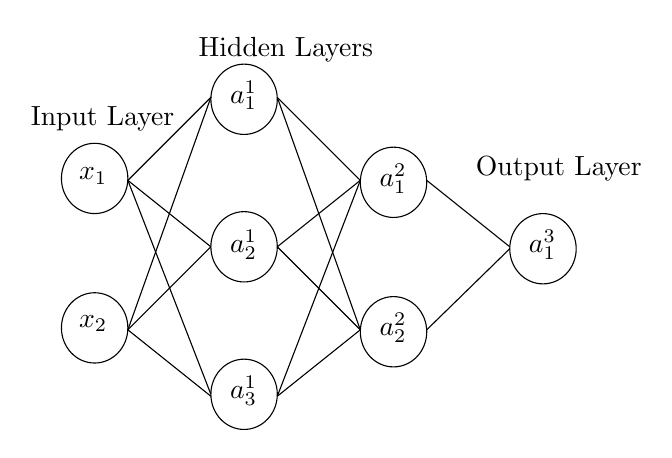
\begin{tikzpicture}[x=0.6pt,y=0.6pt,yscale=-1,xscale=1]
%uncomment if require: \path (0,484); %set diagram left start at 0, and has height of 484

%Flowchart: Connector [id:dp6019250960891445]
\draw  [fill={rgb, 255:red, 255; green, 255; blue, 255 }  ,fill opacity=1 ] (40,112.83) .. controls (40,101.14) and (48.95,91.67) .. (60,91.67) .. controls (71.05,91.67) and (80,101.14) .. (80,112.83) .. controls (80,124.52) and (71.05,134) .. (60,134) .. controls (48.95,134) and (40,124.52) .. (40,112.83) -- cycle ;
%Flowchart: Connector [id:dp8334547170271857]
\draw  [fill={rgb, 255:red, 255; green, 255; blue, 255 }  ,fill opacity=1 ] (40,202.83) .. controls (40,191.14) and (48.95,181.67) .. (60,181.67) .. controls (71.05,181.67) and (80,191.14) .. (80,202.83) .. controls (80,214.52) and (71.05,224) .. (60,224) .. controls (48.95,224) and (40,214.52) .. (40,202.83) -- cycle ;
%Flowchart: Connector [id:dp7153685420206096]
\draw  [fill={rgb, 255:red, 255; green, 255; blue, 255 }  ,fill opacity=1 ] (130,65.17) .. controls (130,53.48) and (138.95,44) .. (150,44) .. controls (161.05,44) and (170,53.48) .. (170,65.17) .. controls (170,76.86) and (161.05,86.33) .. (150,86.33) .. controls (138.95,86.33) and (130,76.86) .. (130,65.17) -- cycle ;
%Flowchart: Connector [id:dp5622283646258179]
\draw  [fill={rgb, 255:red, 255; green, 255; blue, 255 }  ,fill opacity=1 ] (130,154) .. controls (130,142.31) and (138.95,132.83) .. (150,132.83) .. controls (161.05,132.83) and (170,142.31) .. (170,154) .. controls (170,165.69) and (161.05,175.17) .. (150,175.17) .. controls (138.95,175.17) and (130,165.69) .. (130,154) -- cycle ;
%Flowchart: Connector [id:dp16862921724788715]
\draw  [fill={rgb, 255:red, 255; green, 255; blue, 255 }  ,fill opacity=1 ] (130,242.83) .. controls (130,231.14) and (138.95,221.67) .. (150,221.67) .. controls (161.05,221.67) and (170,231.14) .. (170,242.83) .. controls (170,254.52) and (161.05,264) .. (150,264) .. controls (138.95,264) and (130,254.52) .. (130,242.83) -- cycle ;
%Flowchart: Connector [id:dp4149695521858179]
\draw  [fill={rgb, 255:red, 255; green, 255; blue, 255 }  ,fill opacity=1 ] (220,115.17) .. controls (220,103.48) and (228.95,94) .. (240,94) .. controls (251.05,94) and (260,103.48) .. (260,115.17) .. controls (260,126.86) and (251.05,136.33) .. (240,136.33) .. controls (228.95,136.33) and (220,126.86) .. (220,115.17) -- cycle ;
%Flowchart: Connector [id:dp840876892841651]
\draw  [fill={rgb, 255:red, 255; green, 255; blue, 255 }  ,fill opacity=1 ] (220,205.17) .. controls (220,193.48) and (228.95,184) .. (240,184) .. controls (251.05,184) and (260,193.48) .. (260,205.17) .. controls (260,216.86) and (251.05,226.33) .. (240,226.33) .. controls (228.95,226.33) and (220,216.86) .. (220,205.17) -- cycle ;
%Flowchart: Connector [id:dp10784935111712701]
\draw  [fill={rgb, 255:red, 255; green, 255; blue, 255 }  ,fill opacity=1 ] (310,155.17) .. controls (310,143.48) and (318.95,134) .. (330,134) .. controls (341.05,134) and (350,143.48) .. (350,155.17) .. controls (350,166.86) and (341.05,176.33) .. (330,176.33) .. controls (318.95,176.33) and (310,166.86) .. (310,155.17) -- cycle ;
%Straight Lines [id:da7667435970573455]
\draw    (80,114) -- (130,154) ;
%Straight Lines [id:da48448129133283535]
\draw    (170,154) -- (220,114) ;
%Straight Lines [id:da4471635916327932]
\draw    (260,114) -- (310,154) ;
%Straight Lines [id:da5105417767244789]
\draw    (80,204) -- (130,244) ;
%Straight Lines [id:da6281305874976782]
\draw    (170,154) -- (220,204) ;
%Straight Lines [id:da9404110386397875]
\draw    (260,204) -- (310,155.17) ;
%Straight Lines [id:da669909761533326]
\draw    (130,154) -- (80,204) ;
%Straight Lines [id:da03861624272354913]
\draw    (80,204) -- (130,64) ;
%Straight Lines [id:da7865539839743194]
\draw    (80,114) -- (130,64) ;
%Straight Lines [id:da006395151871996019]
\draw    (170,64) -- (220,114) ;
%Straight Lines [id:da6703248416054105]
\draw    (170,64) -- (220,204) ;
%Straight Lines [id:da568582824840071]
\draw    (170,244) -- (220,204) ;
%Straight Lines [id:da5603512527475397]
\draw    (170,244) -- (220,114) ;
%Straight Lines [id:da15589575659778376]
\draw    (80,114) -- (130,242.83) ;

% Text Node
\draw (49,105) node [anchor=north west][inner sep=0.75pt]    {$x_{1}$};
% Text Node
\draw (49,194) node [anchor=north west][inner sep=0.75pt]    {$x_{2}$};
% Text Node
\draw (140,52.33) node [anchor=north west][inner sep=0.75pt]    {$a^{1}_{1}$};
% Text Node
\draw (140,142.33) node [anchor=north west][inner sep=0.75pt]    {$a^{1}_{2}$};
% Text Node
\draw (140,230) node [anchor=north west][inner sep=0.75pt]    {$a^{1}_{3}$};
% Text Node
\draw (230,102.33) node [anchor=north west][inner sep=0.75pt]    {$a^{2}_{1}$};
% Text Node
\draw (230,192.33) node [anchor=north west][inner sep=0.75pt]    {$a^{2}_{2}$};
% Text Node
\draw (320,142.33) node [anchor=north west][inner sep=0.75pt]    {$a^{3}_{1}$};
% Text Node
\draw (20,68) node [anchor=north west][inner sep=0.75pt]   [align=left] {Input Layer};
% Text Node
\draw (288,98) node [anchor=north west][inner sep=0.75pt]   [align=left] {Output Layer};
% Text Node
\draw (185,35) node   [align=left] {\begin{minipage}[lt]{74.80000000000001pt}\setlength\topsep{0pt}
Hidden Layers
\end{minipage}};


\end{tikzpicture}

    \caption{\label{fig: NN Fig} Visual representation of a simple neural network with $2$ inputs, $2$ hidden layers with $3$, $2$ neurons respectively and an output layer with a single neuron.}
\end{figure}

\subsection{Neural Networks}
\noindent
Neural Networks are a class of algorithms in which a set of nodes, often referred to as Neurons, are connected as a weighted graph. Which as the name may suggests, aims to emulate behaviour similar to that of the human brain. Each of the nodes in this graph is then activated by an activation function, which takes the weighted input of all of its connected graphs like
\begin{equation}
    a = \sigma\qty(w_1 a_1' + w_2 a_2' + \dots + w_n a_n' + b)
\end{equation}
where $w_i$, $a_i'$ denotes the weights and activations of the connected nodes, and $\sigma$ the activation function of the node, which is chosen differently depending on the problem at hand. Lastly, we have also have a bias, $b$, which simply shifts the activation of the Node in the case of a binary activation, or tn the case where the activation function is chosen to be the identity function, the bias is simply the intercept.

The simplest type of neural network is the \textit{Feed-Forward Neural Network} (FFNN), which is a directed graph, consisting of layers where every neuron in the preceding layer is connected to every neuron in the following layer as depicted in Fig.~\ref{fig: NN Fig}, which is directed going from left to right.

As the name may suggest, the input layer is where the input data starts out, before being fed forward through the hidden layers of the network, weighted in-between each node before reaching the output layer, the final model. In a similar fashion to other methods of supervised learning, the neural network must first undergo a process of training to obtain a suitable set of weights and biases. This is done by optimizing the all of the weights and biases in the network wrt to a chosen cost function usually by SGD. However, due to the costly nature of evaluating all of these cost functions; an algorithm which cleverly exploits the chain rule of differentiation has been developed to very efficiently compute all of the gradients in the network in a process which is called backpropagation.Neural Networks and Deep Learning

\subsubsection{Backpropagation}
\noindent
We base our explanation of the backpropagation algorithm following more or less directly from \textcite{Nielsen} and \textcite{Mehta_2019}, referring the reader to those texts for the finer details and derivations of how the algorithm actually works, focusing instead on the computational aspects in the present texts. However, in short; the algorithm may be summarized as a clever use of the chain rule of differentiation.

Before we start, we first define a few quantities central to the network. First, we have the set of weights connecting each node in the network
\begin{equation}
    \{w^{1}_{jk}, \dots, w_{jk}^L\}
\end{equation}
where in a somewhat sloppy notation the $j, k$ indices denote the number of neurons in the current and previous layers respectively, thus spanning a different range for each $l$. We also define the set of inputs
\begin{equation}
    \{z_j^1, \dots, z_j^L\}
\end{equation}
which again adheres to the same convention of $j$ denoting the number of neurons in the current layer. These inputs then gets fed into the activation function $\sigma(z_j^l)$ of their corresponding neurons yielding the set of activations
\begin{equation}
    \{a_j^1, \dots, a_j^L\}
\end{equation}
where notably the activation function used in the output layer may differ from the one used in the hidden layers. We denote this special, output activation function as $\tilde \sigma(z_j^L)$.

We then start the backpropagation algorithm by first computing the response of each of the neurons in the network by the Feeding the input data forward in the network, starting with the first hidden layer, which is activated directly by the input data $X_p$ like
\begin{align}\label{eqn: FeedForward Initial}
    \begin{split}
        z^1_j &= w^1_{jk}X_k + b^1_j \\
        a^1_j &= \sigma(z^1_j)
    \end{split}
\end{align}
where we adopt the Einstein summation convention by summing over repeated indices.
We then similarly compute
\begin{align}
    \begin{split}
        z^l_{j} &= w^l_{jk}a^{l-1}_k + b^l_j \\
        a^l_{j} &= \sigma(z^l_{j})
    \end{split}
\end{align}
for hidden layers $l = 2, \dots, L$. Then, for the output layer we compute
\begin{align}
    \begin{split}
        z^{L}_j &= w^{L}_{jk}a^{L-1}_k + b^{L}_j \\
        a^{L}_j &= \tilde\sigma(z^{L}_j)
    \end{split}
\end{align}
where $a^{L}_j$ is the predicted response, and $\tilde\sigma$ is the activation function for the output layer, which as mentioned may differ from the activation function used in the hidden layers.

We then compute the error of the output as
\begin{equation}\label{eqn: delta L}
    \delta^{L}_j = \pdv{C}{a^{L}_{j}} \odot \tilde\sigma'(z^{L}_j)
\end{equation}
where $\odot$ denotes the Hadamard product, which is a form of element-wise multiplication of vectors and matrices. It is also worth to note that Eqn.~\ref{eqn: delta L} implicitly assumes that the derivatives of the output activation function $\pdv{z_j}\sigma(z^l_i) = 0 \enspace \forall \enspace i\neq j$. Whilst this holds true for a wide variety of activation functions; it does not hold for the SoftMax, which we will return to later on when we look at classification.

We then continue on by backpropagating the error like
\begin{equation}
    \delta^{l}_j = \qty(\delta^{l+1}_{k}\qty(w^{l+1})^T_{kj}) \odot \sigma'(z^l_j)
\end{equation}
for all $l = L-1, \dots, 1$.

We may then easily compute the gradients of the cost function wrt. the weights \& biases as

\begin{align}
    \begin{split}
        \pdv{C}{w_{jk}^l} &= \delta_j^l a^{l-1}_k \\
        \pdv{C}{b^l_j} &= \delta_j^l
    \end{split}
\end{align}
which are then used to update the weights and biases via gradient descent. Whilst this is in principle all there is to backpropagation, the way in which this method is performed requires some further modifications when solved on a computer.

\subsubsection{Backpropagation with mini-batches}
\noindent
In order to efficiently perform backpropagation simultaneously across several inputs at once, we need to slightly adjust our algorithm such that we may take advantage of the fast and efficient linear algebra libraries that are available, like in for example Numpy.

We then structure our input and output matrices adhering to the row-major storage of Numpy arrays by letting $X\in[M\times P], \enspace Y\in[M\times Q]$ where $M$ denotes the number of data points in the mini-batch and $P, Q$ the dimensionality of the input and output respectively. Explicitly, our data then undergoes the structure change

\begin{equation}
    X = \qty[
    \begin{matrix}
        X_1 \\ \vdots \\ X_P
    \end{matrix}
    ] \rightarrow
    X = \qty[
    \begin{matrix}
        X_{11} & \dots & X_{1P} \\
                 & \vdots&          \\
        X_{M1} & \dots & X_{MP}
    \end{matrix}
    ]
\end{equation}
similarly, we let $z^l_j \rightarrow z^l_{mj}$ and $a^l_{j}\rightarrow a^l_{mj}$ such that they are in accordance with $X$ and $Y$.

In order to adhere to this new form, we transpose Eqn.~\ref{eqn: FeedForward Initial} which yields
\begin{equation}
    w_{jk}X_K \rightarrow \qty(w_{jk}X_k)^T = X_k^T \qty(w^1)^T_{kj}
\end{equation}
Thus, we may write the initial step as
\begin{align}
    \begin{split}
        z^1_{mj} &= X_{mk}\qty(w^{1})^T_{kj} + b^1_j \\
        a^1_{mj} &= \sigma\qty(z^1_{mj})
    \end{split}
\end{align}
where the transposed bias is implicitly\footnote{Matching the behaviour of Numpys addition operator} added element-wise to each row in the resultant matrix. In a similar fashion, we feed forward for $l = 2, \dots L-1$, the last hidden layer as
\begin{align}
    \begin{split}
        z^l_{mj} &= a^{l-1}_{mk}\qty(w^l)^T_{kj} + b^L_j \\
        a^l_{mj} &= \sigma(z^l_{mj})
    \end{split}
\end{align}
and for the output layer
\begin{align}
    \begin{split}
        z^L_{mj} &= a^{L-1}_{mk}\qty(w^L)^T_{kj} + b^L_j \\
        a^L_{mj} &= \tilde\sigma\qty(z^L_{mj})
    \end{split}
\end{align}
Then, we compute the error of the output error as
\begin{equation}
    \delta^L_{mj} = \pdv{C}{a^L_{mj}} \odot \tilde\sigma'(z^L_{mj})
\end{equation}
which we then backpropagate throughout the layers for $l = L-1, \dots 1$
\begin{equation}
    \delta^{l}_{mj} = \delta^{l+1}_{mk}w^{l+1}_{kj} \odot \sigma'(z^l_{mj})
\end{equation}
and finally for the output layer. We the compute the derivatives of the cost functions wrt. the weights and biases for the input layer
\begin{align}
    \begin{split}
        \pdv{C}{w^{1}_{jk}} &= \qty(\delta^1)^T_{jm} X_{mk} \\
        \pdv{C}{b^1_{j}} &= \sum_m \delta^1_{mj}
    \end{split}
\end{align}
and similarly for layers $l = 2, \dots, L$ as
\begin{align}
    \begin{split}
        \pdv{C}{w^{l}_{jk}} &= \qty(\delta^1)^T_{jm} a^l_{mk} \\
        \pdv{C}{b^l_{j}} &= \sum_m \delta_{mj}
    \end{split}
\end{align}
The derivatives are then used to update the weights and biases by gradient descent in the same way as before. One may also following the same logic optimize for column-major storage, as is used in languages like Fortran, MATLAB, Julia, etc.

\subsubsection{Weight Initialization}
\noindent
For neural networks, particularly larger ones, the way in which the weights may contribute significantly to the convergence of the Network. Where in particular the somewhat naive approach by sampling all the weights in a constant fashion from some normal, or uniform distribution may lead to poor convergence for deeper networks; particularly with a variable number of nodes. Where by virtue of the number of nodes; the product of the weights in one layer may blow up, which in turn will blow up the response of the Network. Several clever schemes are thus employed too initialize the weights in a clever way, which are often specialized to some particular type of Neural Network. One such method is the Xavier initialization, proposed by \textcite{xavier}. In this method, the initial weights are sampled individually for each layer from a uniform distribution\footnote{As a sidenote, some sources suggest it as being sampled from a Gaussian instead. As is seemingly quite common in the ML literature there seemingly no standard practice with a lot of competing conventions. We however, opt to follow the original paper.} bounded by $\pm \sqrt{6/(j + k)}$, where $j, k$ denotes the number of neurons in the current and previous layers respectively. Thus, the magnitude of the initial weights are scaled down with respect to the size of $w^l_{jk}$, thus avoiding the aforementioned problem. Another type of initialization proposed by \textcite{he2015delving} is observed to perform particularly well of a ReLU type activation functions, which we will return to later. In He's initialization method, the weights are sampled from a standard normal distribution $\mathcal N(0, 1)$ scaled down by a factor $\sqrt{2/k}$, where $k$ denotes the number of neurons in the previous layer.

\begin{table*}[]
\caption{\label{tab: activation functions}Various Activation functions used in Neural Networks}
\setlength{\tabcolsep}{20pt}
\renewcommand{\arraystretch}{2.5}
\begin{tabular}{llll}
    Name & Activation Function & Derivative & Range \\
    \hline\hline
    Identity &
    $\sigma(x) = x$  &
    $\sigma'(x) = 1$ &
    $(-\infty, \infty)$
    \\ \hline
    Sigmoid &
    $\sigma(x) = \frac{1}{1 + e^{-x}}$  &
    $\sigma'(x) =\sigma(x)\qty(1-\sigma(x))$ &
    $(0, 1)$
    \\ \hline
    Tanh &
    $\sigma(x) = \tanh(x)$  &
    $\sigma'(x) =  1 - \tanh^2(x)$ &
    $(0, 1)$
    \\ \hline
    ReLU    &
    $\sigma(x) = \left\{\begin{matrix}0 & \text{for } x \leq 0 \\ x & \text{for } 0 < x\end{matrix}\right.$ &
    $\sigma'(x) = \left\{\begin{matrix}0 & \text{for } x \leq 0 \\ 1 & \text{for } 0 < x\end{matrix}\right.$ &
    $[0, \infty)$
    \\ \hline
    LeakyReLU &
    $\sigma(x) = \left\{\begin{matrix}0.01x & \text{for } x \leq 0 \\ x & \text{for } 0 < x\end{matrix}\right.$ &
    $\sigma'(x) = \left\{\begin{matrix}0.01 & \text{for } x \leq 0 \\ 1 & \text{for } 0 < x\end{matrix}\right.$ &
    $(-\infty, \infty)$
    \\ \hline
\end{tabular}
\end{table*}



\subsection{Logistic Regression}
\noindent
As opposed to linear regression where the aim is to project data-points into some linear basis as to model some continuous function, logistic regression instead aims to project data unto some binary response. This may in turn be used classify whether or not some particular data point fits into some category. Thus, we wish to fit our data unto some function $f : \mathbb R \rightarrow [0, 1]$.
\begin{figure}[h!tb]
    \center
    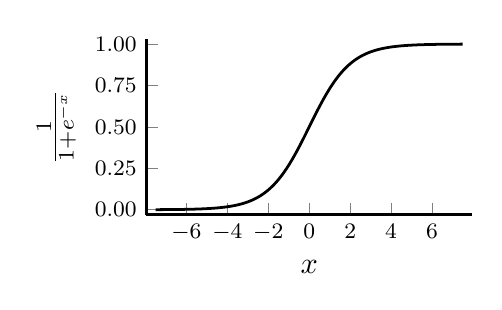
\begin{tikzpicture}[]
\begin{axis}[
  height = {38.1mm},
  ylabel = {$\frac{1}{1 + e^{-x}}$},
  xmin = {-7.95},
  xmax = {7.95},
  ymax = {1.029414054644861},
  xlabel = {$x$},
  unbounded coords=jump,scaled x ticks = false,xlabel style = {font = {\fontsize{11 pt}{14.3 pt}\selectfont}, color = {rgb,1:red,0.00000000;green,0.00000000;blue,0.00000000}, draw opacity = 1.0, rotate = 0.0},xmajorgrids = false,xtick = {-6.0,-4.0,-2.0,0.0,2.0,4.0,6.0},xticklabels = {$-6$,$-4$,$-2$,$0$,$2$,$4$,$6$},xtick align = inside,xticklabel style = {font = {\fontsize{8 pt}{10.4 pt}\selectfont}, color = {rgb,1:red,0.00000000;green,0.00000000;blue,0.00000000}, draw opacity = 1.0, rotate = 0.0},x grid style = {color = {rgb,1:red,0.00000000;green,0.00000000;blue,0.00000000},
draw opacity = 0.1,
line width = 0.5,
solid},axis x line* = left,x axis line style = {color = {rgb,1:red,0.00000000;green,0.00000000;blue,0.00000000},
draw opacity = 1.0,
line width = 1,
solid},scaled y ticks = false,ylabel style = {font = {\fontsize{11 pt}{14.3 pt}\selectfont}, color = {rgb,1:red,0.00000000;green,0.00000000;blue,0.00000000}, draw opacity = 1.0, rotate = 0.0},ymajorgrids = false,ytick = {0.0,0.25,0.5,0.75,1.0},yticklabels = {$0.00$,$0.25$,$0.50$,$0.75$,$1.00$},ytick align = inside,yticklabel style = {font = {\fontsize{8 pt}{10.4 pt}\selectfont}, color = {rgb,1:red,0.00000000;green,0.00000000;blue,0.00000000}, draw opacity = 1.0, rotate = 0.0},y grid style = {color = {rgb,1:red,0.00000000;green,0.00000000;blue,0.00000000},
draw opacity = 0.1,
line width = 0.5,
solid},axis y line* = left,y axis line style = {color = {rgb,1:red,0.00000000;green,0.00000000;blue,0.00000000},
draw opacity = 1.0,
line width = 1,
solid},    xshift = 0.0mm,
    yshift = 0.0mm,
    axis background/.style={fill={rgb,1:red,1.00000000;green,1.00000000;blue,1.00000000}}
,legend style = {color = {rgb,1:red,0.00000000;green,0.00000000;blue,0.00000000},
draw opacity = 1.0,
line width = 1,
solid,fill = {rgb,1:red,1.00000000;green,1.00000000;blue,1.00000000},fill opacity = 1.0,text opacity = 1.0,font = {\fontsize{8 pt}{10.4 pt}\selectfont}},colorbar style={title=},
  ymin = {-0.029414054644860983},
  width = {57.14999999999999mm}
]

\addplot+[
  color = {rgb,1:red,0.00000000;green,0.00000000;blue,0.00000000},
draw opacity = 1.0,
line width = 1,
solid,mark = none,
mark size = 2.0,
mark options = {
            color = {rgb,1:red,0.00000000;green,0.00000000;blue,0.00000000}, draw opacity = 1.0,
            fill = {rgb,1:red,0.00000000;green,0.00000000;blue,0.00000000}, fill opacity = 1.0,
            line width = 1,
            rotate = 0,
            solid
        },forget plot
] coordinates {
  (-7.5, 0.0005527786369235996)
  (-7.4, 0.000610879359434401)
  (-7.3, 0.0006750827306328381)
  (-7.2, 0.000746028833836697)
  (-7.1, 0.0008244246863982953)
  (-7.0, 0.0009110511944006454)
  (-6.9, 0.001006770820085637)
  (-6.8, 0.0011125360328603216)
  (-6.7, 0.0012293986212774202)
  (-6.6, 0.0013585199504289591)
  (-6.5, 0.0015011822567369917)
  (-6.4, 0.0016588010801744215)
  (-6.3, 0.0018329389424928053)
  (-6.2, 0.002025320389049882)
  (-6.1, 0.0022378485212763335)
  (-6.0, 0.0024726231566347743)
  (-5.9, 0.002731960763011059)
  (-5.8, 0.0030184163247084245)
  (-5.7, 0.0033348073074133443)
  (-5.6, 0.003684239899435989)
  (-5.5, 0.004070137715896128)
  (-5.4, 0.004496273160941178)
  (-5.3, 0.004966801650056961)
  (-5.2, 0.005486298899450404)
  (-5.1, 0.006059801491584117)
  (-5.0, 0.0066928509242848554)
  (-4.9, 0.007391541344281971)
  (-4.8, 0.008162571153159897)
  (-4.7, 0.009013298652847824)
  (-4.6, 0.009951801866904324)
  (-4.5, 0.01098694263059318)
  (-4.4, 0.012128434984274237)
  (-4.3, 0.013386917827664779)
  (-4.2, 0.014774031693273055)
  (-4.1, 0.016302499371440946)
  (-4.0, 0.01798620996209156)
  (-3.9, 0.01984030573407751)
  (-3.8, 0.021881270936130476)
  (-3.7, 0.024127021417669196)
  (-3.6, 0.026596993576865856)
  (-3.5, 0.02931223075135632)
  (-3.4, 0.032295464698450516)
  (-3.3, 0.03557118927263618)
  (-3.2, 0.039165722796764356)
  (-3.1, 0.043107254941086116)
  (-3.0, 0.04742587317756678)
  (-2.9, 0.05215356307841774)
  (-2.8, 0.057324175898868755)
  (-2.7, 0.06297335605699649)
  (-2.6, 0.06913842034334682)
  (-2.5, 0.07585818002124355)
  (-2.4, 0.08317269649392238)
  (-2.3, 0.09112296101485616)
  (-2.2, 0.09975048911968513)
  (-2.1, 0.10909682119561294)
  (-2.0, 0.11920292202211755)
  (-1.9, 0.13010847436299786)
  (-1.8, 0.14185106490048777)
  (-1.7, 0.15446526508353473)
  (-1.6, 0.16798161486607552)
  (-1.5, 0.18242552380635635)
  (-1.4, 0.19781611144141825)
  (-1.3, 0.2141650169574414)
  (-1.2, 0.23147521650098238)
  (-1.1, 0.24973989440488234)
  (-1.0, 0.2689414213699951)
  (-0.9, 0.289050497374996)
  (-0.8, 0.31002551887238755)
  (-0.7, 0.3318122278318339)
  (-0.6, 0.35434369377420455)
  (-0.5, 0.3775406687981454)
  (-0.4, 0.401312339887548)
  (-0.3, 0.425557483188341)
  (-0.2, 0.45016600268752216)
  (-0.1, 0.47502081252106)
  (0.0, 0.5)
  (0.1, 0.52497918747894)
  (0.2, 0.549833997312478)
  (0.3, 0.574442516811659)
  (0.4, 0.598687660112452)
  (0.5, 0.6224593312018546)
  (0.6, 0.6456563062257954)
  (0.7, 0.6681877721681662)
  (0.8, 0.6899744811276125)
  (0.9, 0.7109495026250039)
  (1.0, 0.7310585786300049)
  (1.1, 0.7502601055951177)
  (1.2, 0.7685247834990175)
  (1.3, 0.7858349830425586)
  (1.4, 0.8021838885585817)
  (1.5, 0.8175744761936437)
  (1.6, 0.8320183851339245)
  (1.7, 0.8455347349164652)
  (1.8, 0.8581489350995123)
  (1.9, 0.8698915256370021)
  (2.0, 0.8807970779778823)
  (2.1, 0.8909031788043871)
  (2.2, 0.9002495108803148)
  (2.3, 0.9088770389851438)
  (2.4, 0.9168273035060777)
  (2.5, 0.9241418199787566)
  (2.6, 0.9308615796566533)
  (2.7, 0.9370266439430035)
  (2.8, 0.9426758241011313)
  (2.9, 0.9478464369215823)
  (3.0, 0.9525741268224334)
  (3.1, 0.9568927450589139)
  (3.2, 0.9608342772032357)
  (3.3, 0.9644288107273639)
  (3.4, 0.9677045353015494)
  (3.5, 0.9706877692486436)
  (3.6, 0.973403006423134)
  (3.7, 0.9758729785823308)
  (3.8, 0.9781187290638694)
  (3.9, 0.9801596942659225)
  (4.0, 0.9820137900379085)
  (4.1, 0.9836975006285591)
  (4.2, 0.9852259683067269)
  (4.3, 0.9866130821723351)
  (4.4, 0.9878715650157257)
  (4.5, 0.9890130573694068)
  (4.6, 0.9900481981330957)
  (4.7, 0.990986701347152)
  (4.8, 0.9918374288468401)
  (4.9, 0.9926084586557181)
  (5.0, 0.9933071490757153)
  (5.1, 0.9939401985084158)
  (5.2, 0.9945137011005495)
  (5.3, 0.995033198349943)
  (5.4, 0.9955037268390589)
  (5.5, 0.995929862284104)
  (5.6, 0.9963157601005641)
  (5.7, 0.9966651926925867)
  (5.8, 0.9969815836752917)
  (5.9, 0.997268039236989)
  (6.0, 0.9975273768433653)
  (6.1, 0.9977621514787236)
  (6.2, 0.9979746796109501)
  (6.3, 0.9981670610575072)
  (6.4, 0.9983411989198255)
  (6.5, 0.998498817743263)
  (6.6, 0.9986414800495711)
  (6.7, 0.9987706013787226)
  (6.8, 0.9988874639671398)
  (6.9, 0.9989932291799144)
  (7.0, 0.9990889488055994)
  (7.1, 0.9991755753136017)
  (7.2, 0.9992539711661633)
  (7.3, 0.9993249172693672)
  (7.4, 0.9993891206405656)
  (7.5, 0.9994472213630764)
};

\end{axis}

\end{tikzpicture}


    \caption{The logistic function}
\end{figure}

\section{Results \& Discussion}

\begin{figure*}[h!tb]
    \center
    \subfloat{
    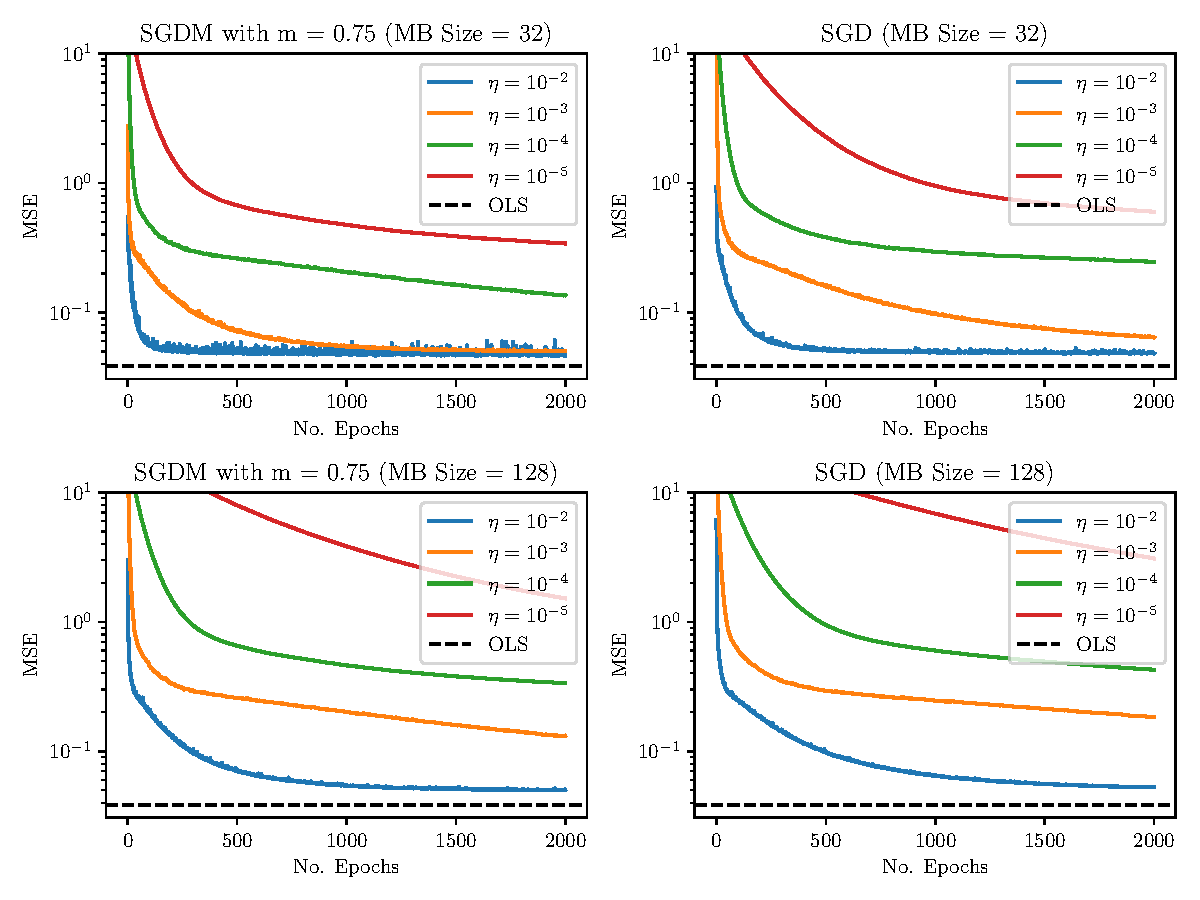
\includegraphics[width=\columnwidth]{SGD_learning_rate.pdf}
    }
    \subfloat{
    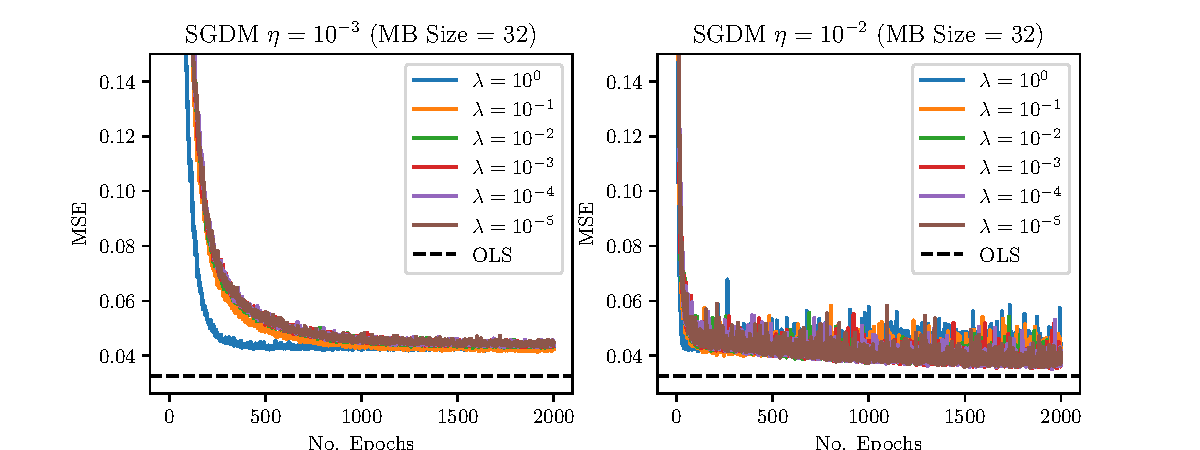
\includegraphics[width=\columnwidth]{SGD_learning_penalty.pdf}
    }
\end{figure*}

\section{Conclusion}

\onecolumngrid
\bibliography{bibfile}
\newpage
\twocolumngrid
\appendix
\end{document}
